\documentclass[a4paper]{jsbook}
%\documentclass[a4paper,oneside]{jsbook} % 片面刷りの場合は oneside を追加
%\documentclass[a4paper,openany]{jsbook} % 章末の白紙ページを省きたいとき

\usepackage[sort]{cite}              % 参考文献のソート
\usepackage[dvipdfmx]{color}
\usepackage{listings}

\renewcommand{\lstlistingname}{リスト}

\definecolor{gray}{rgb}{0.4,0.4,0.4}
\definecolor{darkblue}{rgb}{0.0,0.0,0.6}
\definecolor{cyan}{rgb}{0.0,0.6,0.6}

\lstset{
  basicstyle={\scriptsize\ttfamily},
  columns=fullflexible,
  showstringspaces=false,
  commentstyle=\color{gray}\upshape,
  breaklines=true
}
\lstdefinestyle{normalsize}{
  basicstyle={\ttfamily}
}

\lstdefinelanguage{XML}
{
  morestring=[b]",
  morestring=[s]{>}{<},
  morecomment=[s]{<?}{?>},
  stringstyle=\color{black},
  identifierstyle=\color{darkblue},
  keywordstyle=\color{cyan},
  morekeywords={xmlns,version,type}% list your attributes here
}



\usepackage[mthesis,draft]{salab}    % 草稿では draft を追加
%\usepackage[mthesis]{salab}         % 本番はこっち

\usepackage{comment}

\def\ra{\rightarrow}

\hyphenpenalty=10000

\title{細粒度操作履歴の分析に基づく\\開発行動推薦}
\author{山森 章弘}
\authorintitle{山~~森~~~~~章~~弘} % 表示用
\date{平成28年1月}
\nendo{平成27}
\studentid{14M38439}
\advisor{小林 隆志 准教授}
\affiliation{大学院情報理工学研究科 計算工学専攻}

\begin{document}

\frontmatter
\maketitle

\chapter*{概要}
本論文では,...

\chapter*{Abstract}
This dissertation studies ...

\tableofcontents
\listoffigures
\listoftables

\mainmatter
% 章番号が決まったらファイル名に連番を振っても良いし,
% include せずにすべてをこのファイルに含めても良い.

\chapter{序論}
\section{背景}
ソフトウェアの大規模化に伴い、メンテナンス時のバグ修正や機能追加タスクの作業で必要な依存関係解決の作業量は増大している。
ソフトウェアの品質を向上させるため、メンテナンス作業中に変更の必要なソースコードを全て列挙できることは重要であり、この作業を支援する研究は変更支援(change guide)と呼ばれている。
変更支援のうち、静的解析に基づき、ソースコードの依存関係をもとに変更伝搬箇所を特定する手法が提案されている\cite{792645}が、
この手法は膨大な量の依存関係を解析するため計算量が多く、また全ての依存関係が変更の伝搬を引き起こすわけではないため効率が悪い\cite{Geipel:2009}。
また、静的解析では解決できないようなソフトウェアの依存関係に対しては変更支援を行なうことが出来ない\cite{5609732}。

静的解析による変更支援手法の限界を克服するために、
開発者の過去の開発履歴に注目して開発者に対して変更支援を行なう研究が行われている\cite{738508, Kagdi:2006}。
Zimmermannらは、改版履歴を解析することにより、変更される可能性のあるメソッド、フィールド等のコード要素を推薦する変更推薦ツール、eROSE\cite{Zimmermann:2005}を提案した。

最近では、開発者が過去に操作した統合開発環境(IDE)やWebブラウザ等の開発ツールの情報が記録された操作履歴(interaction history)\cite{rsse:2014}を解析する研究がさかんに行われている。
Sawadskyら\cite{Sawadsky:2013}は、開発者のコードの閲覧と、Webブラウザーを介してAPIのドキュメンテーションページを閲覧する操作を記録し、潜在意味解析(LSA)やTF-IDFを用いて開発者が閲覧すべきドキュメンテーションページを推薦するEclipseプラグイン、Reverbを開発し、被験者実験によってこの推薦のヒット率が高いことを示した。
また、変更支援手法に関する研究\cite{6233415,KatoJapanese:2011,ss2012-76,ss2013-84,Yamamori:2016}では、変更推薦プロセスの性能を向上させるために、ソースコードへの変更と参照の情報を細粒に記録されている操作履歴を変更支援手法に適用した。

細粒度な操作履歴を用いた研究の共通の問題点として、
改版履歴とは異なり操作履歴には一般的に使われている記録ツールが存在せず、
手法の効果の一般性を実証的に示すことが困難なことが挙げられる。
操作履歴を収集するツールにはPLOG\cite{plog}、{\sc DFlow}\cite{minelli:2014}などがあるが、
これらのツールで記録できる操作履歴は取得できる操作の種類や粒度などが異なり、それぞれのツールで記録された操作履歴を相互に変換することはできない。
また、これらのツールの多くは研究目的で製作されたものであり、公開されているものは少ないため、現存する操作履歴は数日〜数週間程度の短いものがほとんどである。

Mylyn\cite{Kersten:2005}は公開されている操作履歴記録ツールであり、実開発で記録された操作履歴が7年分利用可能となっている。
しかし、Mylynで記録された操作履歴は他の細粒度操作履歴と異なり、ファイルの変更を伴う操作かどうかや操作の時系列を復元することが出来ないため、既存の操作履歴を利用した変更支援手法をそのまま適用することが出来ない。
したがって、Mylynで記録された操作履歴を適用できる変更支援手法を確立し変更支援を実行することで、
操作履歴を利用した変更支援が一般の開発作業でも適用可能であることを示すことが必要とされている。
\section{目的}
本稿では、長期間の実開発で記録された操作履歴を利用した変更支援手法の提案を試みる。
この目的のために、以下の2つのアプローチを実行する。
\begin{enumerate}
  \item Mylynを拡張し、既存の変更支援手法に必要な情報を出力できるようにする
  \item 現在までに記録された、Mylynによって記録された操作履歴を利用して、変更支援手法を行えるかどうか検討する
\end{enumerate}
1では、現在広く使われているMylynの機能を拡張し、開発者が変更を行なったかどうかを検知する機能を加え、さらに変更情報と時系列情報を操作の属性として加える拡張を行なう。
この拡張を行なうことで、今後Mylynを利用した実開発プロジェクトにおいて本拡張を適用することにより、実開発の操作履歴に対して、既存の変更支援手法を適用することが可能となり、手法の効果の一般性を実証的に示すことができるようになる。

2では、既存の変更支援手法に必要な情報が欠損したMylynの操作履歴を用いて、変更支援を行える手法について検討する。
Mylynの操作履歴と改版履歴の情報を結合することにより、操作に変更を伴ったかどうかや操作の時系列を擬似的に復元する。
さらに、得られた操作履歴を改版履歴ベースの変更支援手法に適用することで、
実開発において得られた操作履歴が変更支援に有効であるかどうかを検証する。
\section{本論文の構成}
\chapter{関連研究}
\section{変更波及解析による変更支援}
ソースコードの静的解析を用いた変更伝搬箇所特定の研究が行われてきた\cite{792645}。
このような研究では、ソースコードを解析することによって、メソッドコールやクラス継承、フィールド参照等の依存関係を取得している。
しかし、ソフトウェアの内部にはそのような依存関係が無数に存在し、その全てが変更伝搬に関係しているわけではない。
Geipelら\cite{Geipel:2009}は、半分以上のクラス同士の依存関係は変更伝搬に全く関係ない上、ごく一部の依存関係が殆どの変更伝搬に関係していると報告した。
さらに、Canforaら\cite{5609732}は静的解析では一部の依存関係を見つけられないことを報告した。
以上のように、ソースコードの依存関係のみを用いた変更支援は困難であるといわれてきた。

\section{改版履歴をマイニングする手法}
静的解析による変更支援手法の限界を克服するため、ソフトウェア成果物の変更の歴史を利用し、メンテナンス時に必要な変更箇所を推薦するような研究が進められている。

Gallら\cite{738508}はCVSのようなバージョン管理システムに保存された改版履歴を解析し、logical couplingと呼ばれる同時に変更されやすいファイル同士に張られる関係を抽出する手法を提案した。

ZimmermannらはeROSEというツール\cite{Zimmermann:2005}を実装した。
このツールはメソッド粒度でlogical couplingを抽出し、開発者があるメソッドを変更した時に外の変更するべきメソッドを推薦する機能を持つ。
Kagdiらはsqminerというツール\cite{Kagdi:2006}を実装した。
このツールは改版履歴に含まれる変更セットから、logical couplingでは考慮していなかった変更の時系列を擬似的に計算し、変更支援の精度を向上させることに成功した。
Gerardら\cite{5609732}は、グレンジャー因果性検定を使ってバージョン管理システムの改版履歴から相関ルールを抽出し、変更予測を補完する研究を行なった。

これらのCVSやSubversion、Gitなどのようなバージョン管理システムの改版履歴を利用した変更支援の研究は2つの限界が存在する。
1つ目は、バージョン管理システムの改版履歴に保存されるソフトウェア成果物の変更の情報はコミット時のみに記録されるということである。
したがって、変更の発生した正確な時間が改版履歴には記録されない。
2つ目は、改版履歴には変更情報しか記録されず、参照情報が記録されないことである。
参照されたソフトウェア成果物の情報は変更情報と同様に変更支援の情報源となる可能性がある。
\section{操作履歴をマイニングする手法}
改版履歴に代えて、改版履歴よりも細かい粒度で開発者の活動履歴が記録されている操作履歴を保存し、マイニングする手法が提案された\cite{Hill:1992}。
ここで用いられている操作履歴(interaction history)とは、改版履歴でも記録できるファイルの変更の記録だけでなく、選択や参照などの変更を伴わない開発者の操作や、それらの操作の時系列が記録されたものを指す。

本論文では、操作履歴のうち「変更と操作の区別」と操作の正確な時系列が記録されているものを「細粒度操作履歴」と呼び、それ以外を「粗粒度操作履歴」と呼ぶ。
\subsection{細粒度操作履歴をマイニングする手法}
Zouら\cite{4268248}は、メンテナンス作業中のファイルの特徴として、interaction couplingを定義した。
interaction couplingとは、頻繁に同時参照されているファイル間に張られる関係である。
Robbesら\cite{Robbes:2008}も、細粒度操作履歴におけるlogical couplingとして同様の概念を提案した。
彼らは様々な変更予測手法を操作履歴に対して適用し、最近変更されたファイルに基づく手法が最も正確であることを示した\cite{5463278}。

様々な目的で細粒度操作履歴を用いる手法が広く研究されている。
Maalejら\cite{Maalej:2010}は、複数の開発ツールで記録した操作履歴を用いて、
開発者が次に使うべき開発ツールを推薦する手法を提案した。
Roehmらは、コードの変更、Webサーチ、コンパイルエラー等の履歴を収集し、隠れマルコフモデルを用いて開発者が問題解決する段階を表現する過程を可視化した。

小林ら\cite{6233415,KatoJapanese:2011}は、変更と参照の情報が記録された操作履歴を学習して変更支援グラフを作成し、このグラフを基に変更推薦をする手法を提案した。
この研究では、開発者のコードへの参照行為を2つの変更行為の間のコンテクストとして利用し、変更推薦手法の精度を操作履歴によって向上させられることを示した。
さらに、この手法を拡張し,変更間の時間的局所性を考慮した改善手法\cite{ss2012-76}や、
複数箇所に変更が波及する場合を考慮し推薦尤度の累積を行なう手法\cite{ss2013-84,Yamamori:2016}が提案されており、
\cite{Yamamori:2016}では、メソッド粒度の変更推薦において精度が向上することを示した。

細粒度操作履歴を用いて成功している手法の多くは、実証実験を行なうためのデータが不足していることが共通の問題となっている。
これは細粒度操作履歴を記録するためのツールが一般に普及しておらず、多くの研究で実証実験のために記録された短期間の操作履歴を用いているためである。
表\ref{finegrained}は細粒度操作履歴を収集し出力できるツールをまとめたものである。
これらの5つのツールは、開発者の操作を、正確な時間や時系列、変更したかどうかの情報を含めて記録することができる。
この3つの情報はMylynでは記録することができない。

\begin{table}[bt]
  \caption{操作履歴を収集し出力できるツールの一覧}
  \centering
  \begin{tabular}{ll}
    \hline
    ツール名& 操作の種類\\
    \hline
    PLOG\cite{plog} & ファイルへのアクセス、変更の有無\\
           & カーソル行のメソッド名、 標準出力やエラー出力の内容 \\
    FLUORITE\cite{yoon:2011} & ファイルへの挿入や削除、
          コードの行数、 実行等  \\
    CodingTracker & 
    テキストの編集、エディタの比較、 リファクタリング、\\
    \cite{Negara:2012}\cite{Negara:2014}  & 
    バージョン管理システムの操作, 
    JUnitテストの実行、 起動等\\
    {\sc DFlow}\cite{minelli:2014} & コードの読み書き、 ソフトウェア検査等\\
    IDE++\cite{Gu:2014} & キーストローク(キーの名前)、 実行、 \\
                        & リファクタリング、 保存等\\
    \hline
  \end{tabular}
\label{finegrained}
\end{table}

PLOG\cite{plog}は開発者のコードへの参照と編集を、時間と時系列とともに記録するツールである。
また、実行時の実行時例外の発生も記録できる。
YoonらはFLUORITE\cite{yoon:2011}を開発した。
このツールは、ファイルへの挿入や削除、コードの行数や抽象構文木中に含まれるノードの数などを記録でき、また、これらの情報の変化を可視化する機能がある。
この可視化情報をもとに、開発者はソフトウェアの成長過程を見ることができる。
NegaraらはCodingTracker\cite{Negara:2012}という操作履歴記録ツールを実装した。
このツールは、Eclipseのリファクタリング機能の操作などといった38種類のコード進化イベントを記録できる。
彼らは、CodingTrackerを用いて記録された操作履歴を分析し、幾つかのコード変更パターンを見つけ出した\cite{Negara:2014}。
Minelliらは{\sc DFlow}というツールを開発した。
このツールは、PharoというSmalltalk開発用統合開発環境用に実装された操作履歴記録ツールで、Smalltalkの特徴である検査操作などを含む33種類の詳細な操作イベントを記録できる。
彼らは、{\sc DFlow}とPLOGを用いてそれぞれ記録された操作履歴を解析し、開発者のコード理解の段階を明らかにした。
Guらは、キーストロークのような最も細かい粒度で44種類の操作イベントを記録できるツールIDE++\cite{Gu:2014}を開発した。

これらのツールはすべて研究段階にあり、実開発の現場で利用され操作履歴が記録されたものはほとんどない。
したがって、現時点で記録された操作履歴には1年以上の期間記録されたものはないため、数年分の細粒度操作履歴を用いて手法の実証実験を行なうことは非常に困難である。
これは、多くのオープンソースソフトウェアの開発で数年分の改版履歴が記録されており、これを利用して改版履歴を利用した研究が盛んに行われている事実とは対照的である。
\subsection{粗粒度操作履歴をマイニングする手法}
Kerstenらは、開発者が頻繁に操作しているソフトウェア成果物群を検知することで、
現在の開発者が必要としている成果物を特定し集約する手法を提案した。
彼らは、統合開発環境上で集約された成果物を開発者に表示するEclipseプラグイン、``Mylar"(現在の``Mylyn")\cite{Kersten:2005}を実装した。
Mylynは開発者の粗粒度操作履歴を自動で記録する機能が付属している。
Mylynの操作履歴はMylyn自身の開発プロジェクトで2007年から記録が開始され、{\it Bugzilla}上からダウンロード可能となっている。
したがって、Mylynで記録されたこの粗粒度操作履歴を利用して実証実験を行なうことで、前節で挙げた細粒度操作履歴用いる研究の問題を解消することができる。
しかしながら、この粗粒度操作履歴は多くの細粒度操作履歴とは異なり、時間の情報が欠落しており、変更と参照の区別がない( \ref{mylyn_chap} 章を参照)。
細粒度操作履歴を用いた手法に粗粒度操作履歴をそのまま適用させることは出来ないため、粗粒度操作履歴を利用できる新たな手法を生み出す必要がある。

T. Leeら\cite{TLee:2011}はMylynの粗粒度操作履歴を用いた最初の研究を行なった。
彼らは操作履歴をmicro interaction metrics (MIMs)を計算するために利用し、MIMsによって欠陥予測の精度を向上させた。
Blincoeら\cite{Blincoe:2012}はMylynの粗粒度操作履歴を用いて開発者とタスクとの近接度({\it proximity})を求めた。
Robbesら\cite{Robbes:2013}とRicardら\cite{Silva:2015}らも同様にMylynの粗粒度操作履歴から開発者の専門度メトリクスを求めた。
\cite{Blincoe:2012,Robbes:2013,Silva:2015}によってMylynの操作履歴は開発者をタスクに振り分ける際に有効であることが示された。

Zanjaniら\cite{Zanjani:2014}は、変更リクエスト上でテキストマイニング手法を適用し、
Mylynの粗粒度操作履歴のバグ説明文と改版履歴のコミットメッセージを突き合わせることで機能捜索(feature location)を行った。
彼らは、改版履歴とMylynの粗粒度操作履歴の両方を使うことで機能捜索を効率的に行えることを示した。
Zanjaniらの手法はコミットや操作と関係する単語をクエリとして用意する必要があり、変更やコミットをクエリとして変更推薦を行なう本論文の手法とは異なる。

Bantelayら\cite{Bantelay:2013}は、interaction couplingを改版履歴とMylynの粗粒度操作履歴の両方から計算し、両方の履歴を利用することで、それぞれの履歴のみを利用するよりも再現率が向上することを示した。
しかし、この研究には2つの問題点がある。
まず、この研究ではMylynが記録する``selection",``edit",``propagation"などのような操作イベントの種類(\ref{kind_sec}節参照)を考慮せずに全て同一に利用している。
開発者の操作を解析する上では``edit"のイベントのみを利用するべきである。
次に、この研究では、バグのIDのみを用いてMylynの操作履歴とコミットを紐付けている。
Bugzillaにアップロードされた操作履歴には、開発中に記録された操作履歴の他にクラッシュリポートとしてコミットとは全く関係なくアップロードされた操作履歴を含むため、より慎重に操作履歴とコミットを紐付けるべきである。

S. Leeら\cite{SLee:2015}はMylynの粗粒度操作履歴から相関ルールを抽出する推薦システム、{\it MI}を、eROSE\cite{Zimmermann:2005}を拡張することで開発した。
彼らはMylynのselectionイベントをコードへの参照として、editイベントをコードへの変更としてそれぞれ利用した。
しかし、実際にはeditイベントは開発者がコードを見るだけで発生し、コードが変更されたかどうかとは関係がないため、この点について正しく解釈した研究が必要とされている。

\chapter{Mylynの操作履歴}\label{mylyn_chap}
Mylyn\cite{Kersten:2005}はタスクマネージメントツールであり、Eclipseプラグインとして実装されている。
MylynはEclipseに標準でバンドルされているため、既に多くの開発者にMylynが配布されている。
Mylynの主な機能はタスクに関係するファイルを集約することだが、この機能に付随して、タスクが活性化されている間、開いたファイルの情報やカーソルの移動の情報等を操作イベントとして記録し、XML形式のログファイルに出力する機能がある。
本稿では、このログファイルのことを``Mylynログ"と呼び、あるタスクを実行中に記録された操作の列を``セッション"、セッションの列を``(Mylynの)操作履歴"と呼ぶ。
また、それぞれのセッションに含まれる1つの操作を``操作イベント"と呼ぶ。

MylynプロジェクトはイシュートラッキングシステムであるBugzilla\footnote{\url{https://bugs.eclipse.org/bugs/}}を利用している。
MylynプロジェクトのすべてのコミッターはMylynを用いてBugzillaにMylynログをアップロードする義務を負っているため\footnote{\url{https://wiki.eclipse.org/Mylyn/Contributor_Reference\#Using_Mylyn}}、Mylynログは2007年からBugzilla上にアップロードされ続け、現存する最も長期間の操作履歴となっている。

図\ref{bugzilla_webpage}は、Mylynプロジェクトが利用しているBugzillaのページの一例である。
この図の左側中段にある"mylyn/context/zip"というリンクをクリックすることでMylynログをダウンロードすることが可能である。

\begin{figure}[tb]
  \centering
  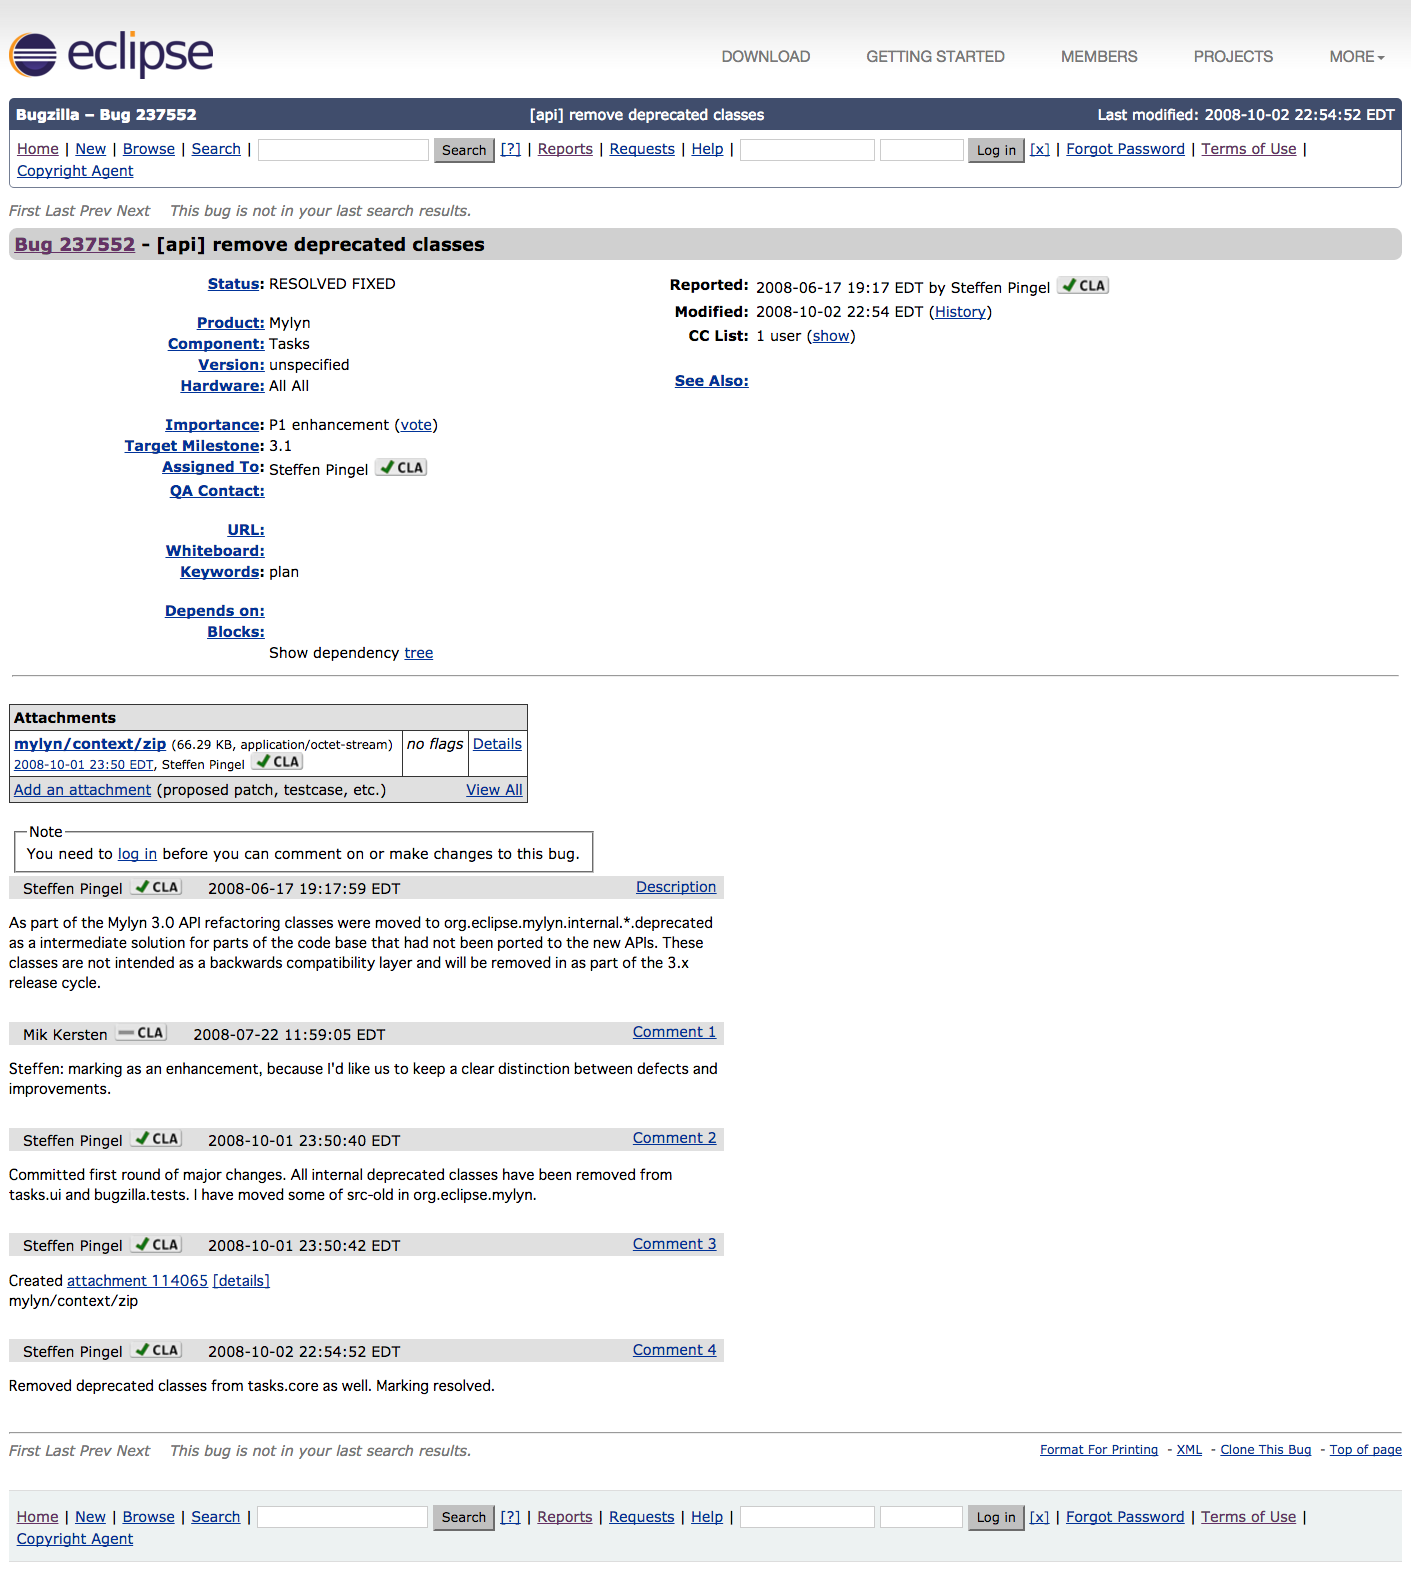
\includegraphics[width = \linewidth]{resource/bugzilla_webpage.png}
  \caption{MylynログがアップロードされているBugzillaのページの例 (\url{https://bugs.eclipse.org/bugs/show_bug.cgi?id=237552})}
  \label{bugzilla_webpage}
\end{figure}


操作イベントはXMLの要素で表され、{\it Kind}、{\it StructureHandle}などの属性が存在する。
以下の節ではそれぞれの属性について詳しく説明する。

\section{Kind}\label{kind_sec}
{\it Kind}属性はすべての操作イベントに対して記録され、イベントの種類を表している。
{\it Kind}のリストを表\ref{kind_table}に表す。
表に含まれる{\it Kind}のうち、``command"、``preference"、``attention"の3つは、Mylynが内部的に持っているのみでファイルには書き出されない。

先行研究\cite{6233415,KatoJapanese:2011,ss2012-76,ss2013-84,Yamamori:2016}の手法では変更を伴う操作と変更を伴わない操作を区別する必要があるが、Mylynログにはこの情報が記録されていないため、Mylynログをこれらの手法に適用することは出来ない(図 \ref{mylyn_interaction})。

本稿においては、エディタのカーソル位置を開発者が閲覧しているコードとみなせることから、{\it Kind}が``edit"であるような操作イベントは開発者がコードを閲覧していると解釈し、そのような操作イベントを利用して開発者が閲覧しているコードを特定する。
また、{\it Kind}が``edit"以外である操作イベントは本稿では利用しない。

\begin{table}[tb]
  \centering
  \caption{Mylynによって記録される{\it Kind}の一覧}
  \label{kind_table}
\begin{tabular}{ll}
  \hline
  Kind & 概要\\
  \hline
  selection & ファイルオープン、タブ切り替え\\
  edit & エディタ上でのカーソル位置 (コードをエディットしたかどうかを問わない)\\
  propagation & パッケージエクスプローラー上での成果物名のクリック操作\\
  command & ボタンのクリック、 キーショートカットの実行など\\
  preference & ワークベンチの設定の変更\\
  prediction & 開発者が行う可能性のある操作の予測\cite{Kersten:2006}\\
  manipulation & Mylynのタスクコンテクストに手動で成果物を追加する操作\\
  attention & タスクの活性化と非活性化\\
  \hline
\end{tabular}
\end{table}

\section{Date}\label{date_sec}
操作イベントには、"{\it StartDate}","{\it EndDate}"の2つの時間に関する属性がある。
これらはそれぞれ、タスクを活性化させている期間全体での最初のタイムスタンプと最後タイムスタンプを表現している。
操作履歴がMylynログに出力される際、開発者の操作は、成果物名と{\it Kind}の組に対して1つの操作イベントに集約される(図\ref{mylyn_interaction})。
この集約機能により、開発者が実際に成果物を閲覧した正確な時間や順序の情報は欠落してしまい、復元することができなくなる。
図\ref{mylyn_interaction}を例にとり、開発者が「$A\ra C \ra A \ra B \ra C \ra A$」の順にファイルを閲覧した場合を考える。
この場合、Mylynログにはそれぞれの成果物を閲覧した最初の時刻と最後の時刻が{\it StartDate},{\it EndDate}であり{\it Kind}が``edit"であるような操作イベントが記録される。
この操作イベントから、もとの閲覧順序を復元することはできなくなっている。
したがって、成果物への操作の順序が重要である先行研究\cite{6233415,KatoJapanese:2011,ss2012-76,ss2013-84,Yamamori:2016}の手法にMylynの操作履歴を適用することは出来ない。
\begin{figure}[tb]
  \centering
  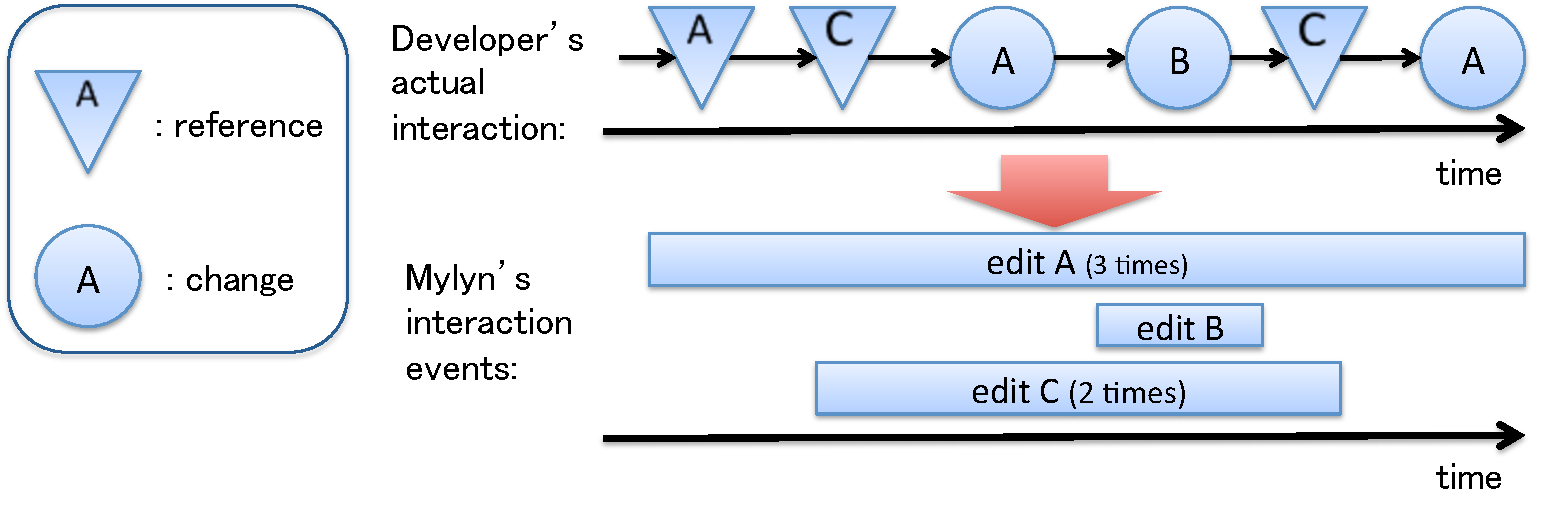
\includegraphics[width = \linewidth]{resource/mylyn_interaction.pdf}
  \caption{Mylynで記録される操作イベントの概略}
  \label{mylyn_interaction}
\end{figure}
\section{StructureHandle}
{\it StructureHandle}は操作イベント発生時に操作されたソフトウェア成果物を表す属性であり、すべての操作イベントに記録される。
{\it StructureHandle}には、``Java要素"、``jarファイルに含まれるJava要素"、``その他の要素"の3つの種類が存在する。
これらの3つの種類の成果物は、{\it StructureHandle}の文字列表現のフォーマットがそれぞれ異なる。

Java要素についてはMylynのオリジナルのフォーマッティングルールが適用され、プロジェクト、パッケージ、ファイル、クラス、メソッド、フィールドのうちのいずれかの粒度で記録される。
ここで、Mylynによって記録される成果物の粒度は各操作に対し1つのみであることに注意が必要である。
例えば、ある操作イベントがコード上のメソッドブロック内で発生した場合、この操作はメソッドの粒度のみで記録され、このメソッドを含むクラス、ファイル、パッケージ、プロジェクトの粒度では記録されない。
したがって、クラスに対する操作イベントは、メソッドブロックまたはフィールド行以外の部分で操作イベント発生した時のみ記録され、同様にファイルに対する操作イベントは、クラスブロックの外で操作イベントが発生した場合のみに記録される。

Java要素を表す{\it StructureHandle}の例として、``=W/src$<$X\{Y.java[Y$\sim$z$\sim$I"という{\it StructureHandle}を考える。
\begin{comment}
]%Vimプラグインが暴れないためのおまじない
\end{comment}
これは、「{\it z(int arg)}」という名前のメソッドが操作されたことと、このメソッドが、「{\it W}プロジェクトの中の{\it src}というソールフォルダ内にある{\it X}パッケージの{\it Y.java}というソースファイルの{\it Y}クラス」内にあることを示す。
引数の{\it I}の部分はEclipseのSignatureシンタックス\footnote{\url{http://help.eclipse.org/mars/topic/org.eclipse.jdt.doc.isv/reference/api/org/eclipse/jdt/core/Signature.html}}である。

jarファイルに含まれるJava要素については、通常のJava要素と似たフォーマッティングルールで記録される。
その他のファイルについては、プロジェクトルートの相対パスが"/"区切りでそのまま記録される。

本稿では、\ref{experiment_chap}章の実験においては、{\it StructureHandle}が通常のJava要素を表し、かつファイルレベルまたはメソッドレベルであるような操作イベントのみを用いる。

\section{NumEvent}
{\it NumEvent}は、集約した操作イベントの個数を表す数値であり、Mylyn 3.0.3で導入された。

Mylynの内部では操作イベントが頻繁に発生している。
{\it Kind}が``edit"である操作イベントは、開発者が「エディタ上でカーソルを動かした後カーソルを一定時間(1秒程度)止める」という動作を行なうたびに発生する。
Mylynではこのように発生した操作イベントを1つに集約する際、いくつの操作イベントを集約したかを{\it NumEvent}という属性で記録している(図\ref{mylyn_interaction})。
\section{Interest}
{\it Interest}とは、Mylynエンジンが計算する成果物に対する開発者の興味の度合い(Degree of Interest, DoI)であり\cite{Kersten:2006}、少なくともMylynの最初のメジャーリリースより前の時点で実装されたものである。
この属性は、対象とする成果物を操作するたびに急激に増加し、対象とする成果物以外を操作するとゆるやかに減少するような指標であり、
「タスクに関係する成果物の集約」というMylynの主機能の実現のために使われている。

\chapter{Mylynの操作履歴を細粒度にする拡張}\label{mylynplus_chap}
\section{概要}
本章では、開発者が変更を行なったかどうかを検知する機能と、変更情報と時系列情報を操作の属性として加えてMylynログに出力する機能をMylynに加える拡張について述べる。

多くの操作履歴収集ツール(表\ref{finegrained})は、操作の順序や変更の有無の情報などを含む細粒度の操作履歴を取得することができ、これらの情報を用いた変更支援手法の研究では一定の成果を上げている。
しかし、これらの操作履歴取得ツールは一般に普及しておらず、
実証実験に用いるためのデータセットを収集することが困難である。
\cite{6233415,KatoJapanese:2011,ss2012-76,ss2013-84,Yamamori:2016}ではデータセット収集のために、15人の被験者に対し2週間程度の開発を行わせることで操作履歴を取得しているが、人数、期間が小さいことや実製品の開発で取得した操作履歴ではないことから、より一般的なデータセットを利用する必要がある。

一方、Mylyn\cite{Kersten:2005}は一般の開発者に配布されているタスクマネジメントツールであり、操作履歴の取得が可能である。
MylynはEclipseに標準でインストールされており、Mylyn自身の開発プロジェクトにおいて現在までに7年分の操作履歴が記録されているなど多くの開発プロジェクトでMylynが使われていることから、この操作履歴を利用することでより一般的な実証実験を行なうことが可能となる。
しかし、Mylynの記録する操作履歴(Mylynログ)は操作の順序(\ref{date_sec}節)や変更の有無(\ref{kind_sec}節)が記録されておらず、既存の変更支援手法にこの操作履歴を適用することが出来ない。

Mylynログを用いて既存の変更支援手法を実施するために、Mylynの出力する操作履歴に細粒度の情報を付け加える拡張を行なうことを考える。
これを実施することで、既に広く配布されているMylynプラグインを利用しているプロジェクトにおいて、より長期間、大人数、かつ実製品の開発で記録された細粒度操作履歴を取得できるようになる。

\section{設計}
Mylynに対して次の3点の拡張を行なうことで、前節で述べた情報をMylynログに加える。
\begin{enumerate}
  \item 変更を伴う操作かどうかの情報を記録する
  \item カーソルがある成果物から別の成果物に移るたびに、カーソルが成果物の中に入った時刻、出た時刻の情報と、この期間に変更を伴ったかどうかを記録する
  \item {\it Kind}が"edit"である操作イベントに以上の情報を加えて、ファイル出力する
\end{enumerate}
機能1は、{\it Kind}が"edit"である操作イベントが発生するたびにその成果物が含まれているファイルの内容を取得し、直前の操作イベントと比べファイルの内容が変化していた場合は「変更した("modified")」、そうでない場合は「参照した("referred")」として操作イベントに情報を付け加えるで実現した。
ただし、直前の操作イベントと比べ成果物名({\it StructureHandle})が変化していた場合はカーソルが成果物間を移動したことを示しているため、ファイルの内容の変化にかかわらず「参照した」扱いとする。
また、Mylynのタスクを活性化した直後の操作イベントは、直前の操作イベントがないため「参照した」扱いとする。
ファイルを保存する前のファイルの内容を取得する必要があるため、ファイルの内容の取得はファイルシステムからではなく、Eclipseのエディターから取得している。
また、ファイルの比較は変更されたかどうかの2択で良いため、ファイルの内容をJavaのStrint\#hashCode()メソッド\footnote{\url{https://docs.oracle.com/javase/8/docs/api/java/lang/String.html\#hashCode--}}でハッシュ化してから比較して、高速化を図った。

機能2のうち時刻については、{\it Kind}が"edit"である操作イベントが発生するたびに直前の操作イベントの成果物名を比較し、変化していた場合は、直前の操作イベントの時刻を直前の操作イベントの成果物からカーソルが離れた時刻、今発生した操作イベントの時刻をその成果物にカーソルが入った時刻として記録することで実現する。
ただし、Mylynのタスクを活性化した直後の操作イベントは、直前の操作イベントがないためカーソルが成果物に入った時刻のみを記録する。
さらに、Mylynが非活性化した時は、直前の操作イベントの成果物からカーソルが離れたとみなしてその時刻を記録する。
機能2のうち変更を伴ったかどうかについては、カーソルが成果物に入った時刻から出た時刻までの間に「変更した」と記録されている操作イベントが1つでも存在する場合は「変更した」、すべての操作イベントが「参照した」ならば「参照した」とすることで実現する。

機能3では、Mylynログに操作履歴を書き出す際にInteractionEventという要素に{\it DurationList}という属性を追加し、その属性値として機能2で得た情報を書き込むことで実現する。
{\it DurationList}の形式をBNF記法で以下に示す。
\begin{verbatim}
  <DurationList> ::= "[" + { <Duration> + "," } * + <Duration> "]"
  <Duration> ::= <Date> + "/" <Date> + "/" + <Ismodified>
  <Date> ::= ("yyyy-MM-dd HH:mm:ss.S z"の形式で表現された時刻)
  <Ismodified> ::= "modified" | "referred"
\end{verbatim}
ここで、\texttt{<Duration>}に含まれる2つの{\texttt{<Date>}のうち、1つ目はカーソルが成果物に入った時刻を、2つ目はカーソルが成果物から出た時刻を表す。
また、\texttt{<DurationList>}は\texttt{<Duration>}を時系列順に並べたものである。
\section{実行例}
本拡張によって記録されるMylynログの例として、著者が\ref{experiment_chap}章で実装した実験コードを編集する際に記録したMylynログから、{\it DurationList}が含まれるInteractionEventのうち2つをリスト\ref{durationlist_fig}に示す。
なお、このMylynログ全体は付録\ref{mylyn_log_appendix}に掲載する。

\begin{lstlisting}[style=normalsize, language=xml, caption=拡張されたMylynによって記録されたMylynログの例(ただしXML上で実体参照に変換された文字はもとに戻している), label=durationlist_fig]
<InteractionEvent Delta="null" EndDate="2016-01-12 17:03:06.423 JST" Interest="15.0" Kind="edit" Navigation="null" OriginId="org.eclipse.jdt.ui.CompilationUnitEditor" StartDate="2016-01-12 16:38:31.648 JST" StructureHandle="=MylynGitPrediction/src<tkobaya.yamamori.mgprediction.combine{MylynReaderResult.java[MylynReaderResult~ addInteractionSet~QMylynInteractionHistory;~D" StructureKind="java" NumEvents="15" CreationCount="103" DurationList= "[2016-01-12 16:38:31.648 JST/2016-01-12 16:40:16.482 JST/modified, 2016-01-12 17:02:58.409 JST/2016-01-12 17:03:06.423 JST/modified]"/>

<InteractionEvent Delta="null" EndDate="2016-01-12 16:52:53.826 JST" Interest="29.0" Kind="edit" Navigation="null" OriginId="org.eclipse.jdt.ui.CompilationUnitEditor" StartDate="2016-01-12 16:43:09.833 JST" StructureHandle="= MylynGitPrediction/src<tkobaya.yamamori.mgprediction.combine{SingleFileSet.java[SingleFileSet~putAll~QMap<+QInteger;+QDouble;>;" StructureKind="java" NumEvents="29" CreationCount="157" DurationList=" [2016-01-12 16:43:09.833 JST/2016-01-12 16:43:11.666 JST/referred, 2016-01-12 16:51:14.131 JST/2016-01-12 16:51:14.131 JST/referred, 2016-01-12 16:51:38.25 JST/2016-01-12 16:52:53.826 JST/modified]"/>
\end{lstlisting}

1つ目の操作イベントは、{\it Kind}が"edit"であることからカーソル移動に関する操作があったことがわかり、
{\it StructureHandle}から、"MylynGitPrecition"というプロジェクトの中にある"tkobaya.yamamori.mgprediction.combine"パッケージの"MylynReaderResult.java"に実装されている"MylynReaderResult\#addInteractionSet( MylynInteractionHistory a, double b)
\footnote{メソッドの仮引数名は記録されないため、ここではa, b, \dots とする}"というメソッドに対する操作であることがわかる。
また、{\it StartDate}と{\it EndDate}からこのメソッドは2016年1月12日16時38分31秒648(日本標準時)に初めてカーソルが入り、同日の17時3分6秒423を最後にカーソルがこのメソッドに入ることはなかったことがわかる。
同様に2つ目の操作イベントは、"SingleFileSet\#putAll( Map<Integer,Double> a)"というメソッドにカーソルが入ったことを表し、その最初の時刻は16時43分09秒833、最後の時刻は16時52分53秒826であった。
したがって、以上のDurationListを含まない情報からこれらのメソッドは16時43分から53分ごろまでの10分間はどちらもカーソルが入っていた可能性がある。
しかし、この情報のみでは、2つのメソッドにカーソルが入った順番の情報を復元することが出来ない(図\ref{only_startdate_enddate})。

\begin{figure}[tb]
  \centering
  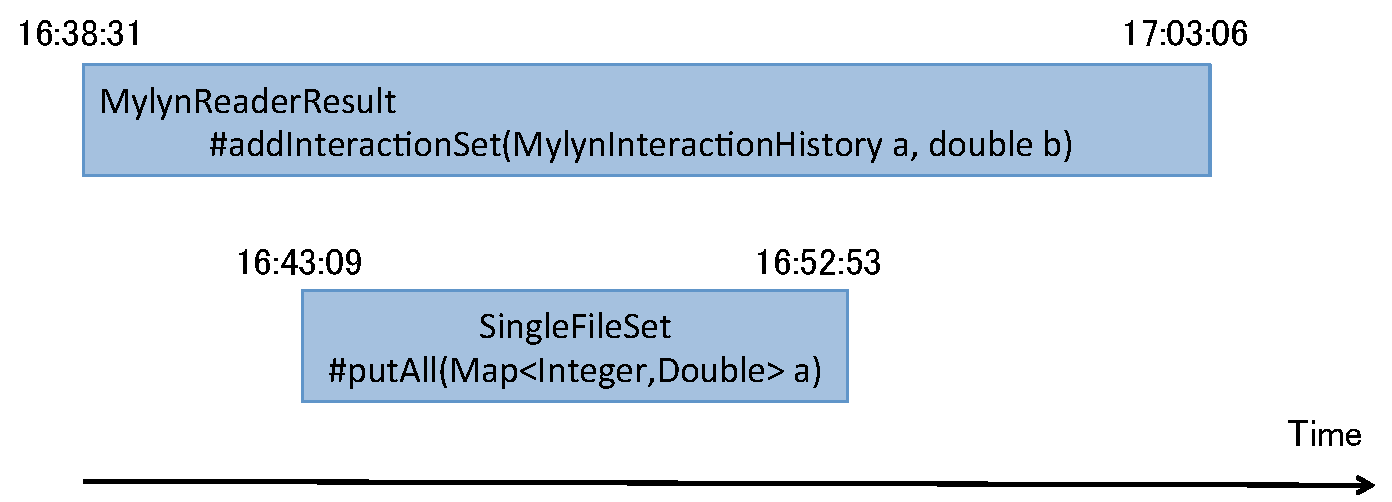
\includegraphics[width = \linewidth]{resource/only_startdate_enddate.pdf}
  \caption{拡張前のMylynログでは、カーソルの移動した順序を復元することが出来ない}
  \label{only_startdate_enddate}
\end{figure}


本拡張で追加した{\it DurationList}について注目すると、"addInteractionSet()"メソッドには16時38分31.648秒〜16時40分16秒482と17時2分58秒409〜17時3分6秒423の2回カーソルが入っており、
"putAll()"には16時43分9秒833〜16時43分11秒666と、16時51分14秒131、16時51分38秒〜16時52分53秒826の3回カーソルが入ったことがわかる。
したがって、これら2つのメソッドのみについて考えると、カーソルの移動した順序は
"addInteractionSet()" $\Rightarrow$
"putAll()" (3回) $\Rightarrow$
"addInteractionSet()"
であることがわかる(図\ref{with_durationlist})。

また、カーソルが入ってから出るまでに変更を伴ったかどうかについても記録されており、"addInteractionSet()"の2回のカーソル移動では変更を伴っていること、"putAll()"の3回のカーソル移動のうち、1回目2回目は変更が行われておらず、3回目のみ変更が行われていることがわかる(図\ref{with_durationlist})。

\begin{figure}[tb]
  \centering
  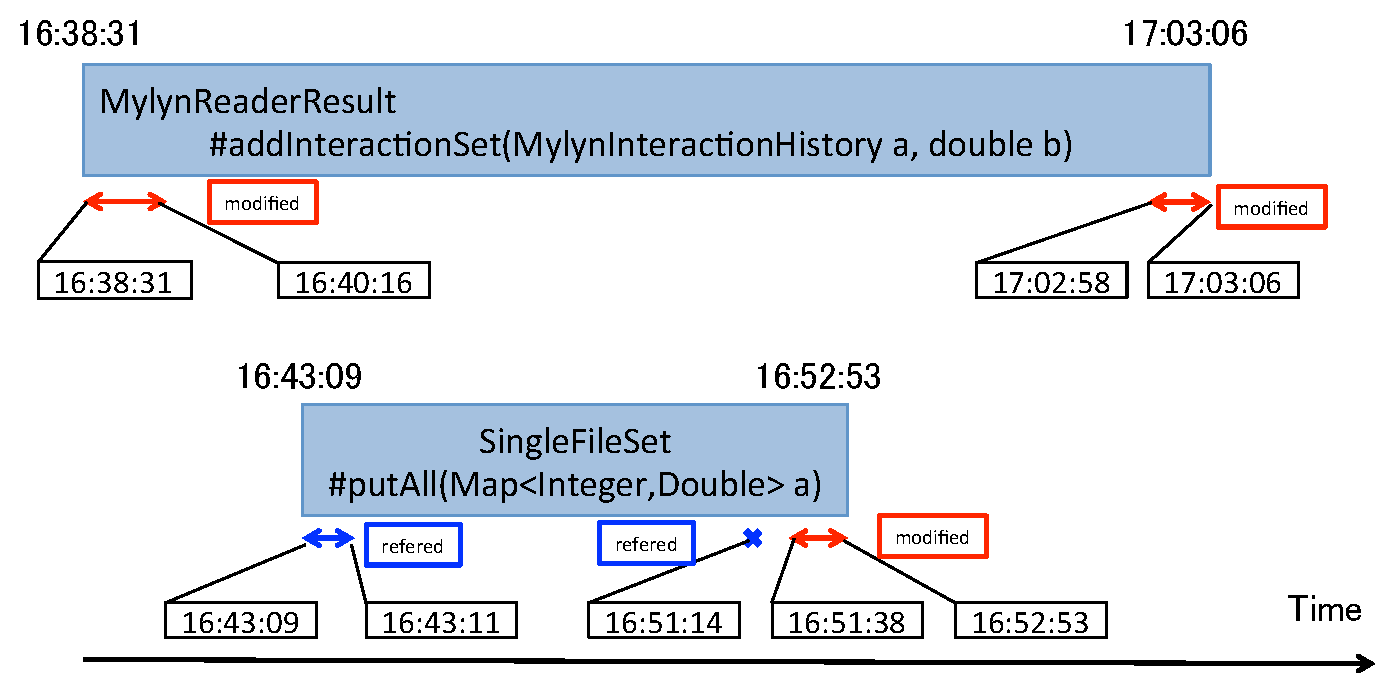
\includegraphics[width = \linewidth]{resource/with_durationlist.pdf}
  \caption{拡張後のMylynログでは、カーソルの移動した順序を復元でき、変更の有無も記録される}
  \label{with_durationlist}
\end{figure}

以上のようなMylynの拡張を行なうことで、
\cite{6233415,KatoJapanese:2011,ss2012-76,ss2013-84,Yamamori:2016}の手法に対してMylynログを適用することができるようになる。

\chapter{Mylynの操作履歴による変更推薦}\label{experiment_chap}
\section{概要}
\ref{mylynplus_chap}章では、今後記録されるMylynログに細粒度な操作の情報を付け足すことで、既存の細粒度操作履歴を用いる変更支援手法にMylynログを適用するアプローチを採用した。
本章では、Mylynログに細粒度な情報を付け足すことなく、これまでに記録されたMylynログを用いて変更支援を行なえるかどうかを調査する。

コード要素の変更情報を取得するため、Mylynの操作履歴をGitの改版履歴と突合し、擬似的な細粒度操作履歴を作成する。
そして、擬似細粒度操作履歴を既存の改版履歴ベースの変更推薦手法に適用することで、Mylynの操作履歴が変更推薦に適用できるか否かを検証する。
検証の際は、既存の改版履歴ベースの変更推薦手法に改版履歴を適用する従来の手法を比較対象とし、推薦精度が向上しているかを確認する。

実証実験は以下の4段階で行なう(図\ref{procedure})。
\begin{enumerate}
  \item 改版履歴と操作履歴を取得する
  \item 得られた改版履歴と操作履歴を突合する
  \item 相関ルールを抽出する
  \item メトリクスを用いて相関ルールの質を評価する
\end{enumerate}
\begin{figure}[tb]
  \centering
  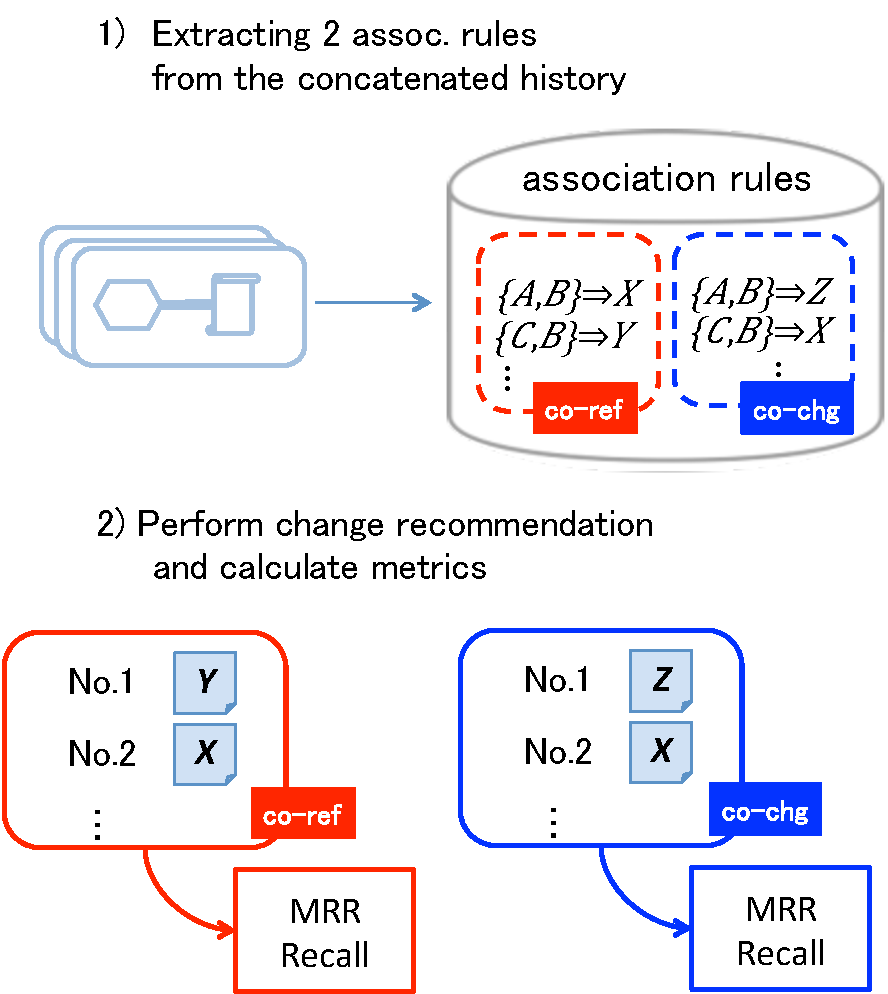
\includegraphics[width = \linewidth]{resource/procedure.pdf}
  \caption{Experimental process}
  \label{procedure}
\end{figure}




\section{操作履歴の取得}
\section{改版履歴と操作履歴の結合}
\section{相関ルールの抽出}
\section{評価メトリクス}
\chapter{評価実験}
%section分け未定
\chapter{結論}
\chapter*{謝辞}
\appendix
\chapter{拡張したMylynによって取得できる操作履歴ログファイルの例}\label{mylyn_log_appendix}
\lstinputlisting[language=xml]{local-2.xml}
%\chapter{付録B}

\backmatter
\bibliographystyle{junsrt}
\bibliography{bibtex/citation}
% 最終稿段階で .bbl に細かい修正を入れること.

\end{document}
